% !TeX spellcheck = en_US 
\documentclass[11pt]{article}

\usepackage{amssymb} % see: http://milde.users.sourceforge.net/LUCR/Math/mathpackages/amssymb-symbols.pdf
\usepackage{mathtools} % for extended mathematical symbols and more

% Page properties :
% See : https://tex.stackexchange.com/questions/36085/latex-without-pages
\usepackage{geometry}
\geometry{margin=16mm}

\usepackage{caption}

\usepackage{wrapfig}


% fix for underlined text not hyphenating :
%\usepackage{soul} % use this
% then replace '\underline{}' with '\ul{}'

% To color text :
% see : https://en.wikibooks.org/wiki/LaTeX/Colors
\usepackage[dvipsnames]{xcolor} % use this
% then use one of these syntaxes :
% >\textcolor{declared-color}{text}
% >{\color{declared-color} text}

% Input file encoding :
\usepackage[utf8]{inputenc}     % makes accents not shit

% To use images : 
\usepackage{graphicx} % use this
\graphicspath{ {./IMG/} } % path midifier for storing images
% to include a picture, type this ('name' is without path or extention) :
% \includegraphics[width=0.5\textwidth]{name}

% Box : % width should be manually set
% \fbox{ \parbox{0.8\textwidth}{ text } }

% Espacement :
% \hfill \vfill
% \vspace{length} \hspace{length} % if ignored, use starred version or { \vspace*{length} }
% \phantom{text} 
% Indentation explicite :
% \indent et \noindent
\usepackage{parskip}

% Fractions :
% \frac{num}{denum}  % small text num/denum
% \dfrac{num}{denum} % normal text num/denum

% Coloring text: % works on text and math modes
% \textcolor{declared-color}{text}
% {\color{declared-color}some text}

% How to use references :
\usepackage{hyperref} % use this
% use '\hypertarget{some_label}{}', then
% and reference it with '\hyperlink{some_label}{some text}'
\hypersetup{
	colorlinks=true,    
	urlcolor=blue,
}

% To write prooftrees :
% see : http://www.pirbot.com/mirrors/ctan/macros/latex/contrib/ebproof/ebproof.pdf
%\usepackage{ebproof} % use this


% Verbatim blocks :
\usepackage{verbatim} % normal verbatim
\usepackage{fancyvrb} % for fancy boxed varbatims
\usepackage{parskip}

% For code
\usepackage{listings}
%\begin{lstlisting}
%Put your code he<re.
%\end{lstlisting}


\usepackage{color}

\definecolor{mylightgray}{rgb}{0.95,0.95,0.95}
\definecolor{mygreen}{rgb}{0,0.6,0}
\definecolor{mygray}{rgb}{0.5,0.5,0.5}
\definecolor{mymauve}{rgb}{0.58,0,0.82}

\usepackage[super]{nth}

% Regulates \tableofcontents max depth
\setcounter{tocdepth}{2}

\usepackage{array}
\newcolumntype{L}[1]{>{\raggedright\let\newline\\\arraybackslash\hspace{0pt}}m{#1}}
\newcolumntype{C}[1]{>{\centering\let\newline\\\arraybackslash\hspace{0pt}}m{#1}}
\newcolumntype{R}[1]{>{\raggedleft\let\newline\\\arraybackslash\hspace{0pt}}m{#1}}

\usepackage{xcolor,colortbl}
\newcolumntype{a}{>{\columncolor{mylightgray}}l}

\usepackage{array}
\setlength\extrarowheight{4pt} % or whatever amount is appropriate

\lstset{ 
	backgroundcolor=\color{mylightgray},   % choose the background color; you must add \usepackage{color} or \usepackage{xcolor}; should come as last argument
	basicstyle=\small,        % the size of the fonts that are used for the code
	breakatwhitespace=false,         % sets if automatic breaks should only happen at whitespace
	breaklines=true,                 % sets automatic line breaking
	captionpos=b,                    % sets the caption-position to bottom
	commentstyle=\color{mygreen},    % comment style
	deletekeywords={...},            % if you want to delete keywords from the given language
	escapeinside={\%*}{*)},          % if you want to add LaTeX within your code
	extendedchars=true,              % lets you use non-ASCII characters; for 8-bits encodings only, does not work with UTF-8
	firstnumber=1,                % start line enumeration with line 1000
	frame=single,	                   % adds a frame around the code
	keepspaces=true,                 % keeps spaces in text, useful for keeping indentation of code (possibly needs columns=flexible)
	keywordstyle=\color{blue},       % keyword style
	%language=Java,                 % the language of the code
	morekeywords={},            % if you want to add more keywords to the set
	numbers=none,                    % where to put the line-numbers; possible values are (none, left, right)
	numbersep=5pt,                   % how far the line-numbers are from the code
	numberstyle=\tiny\color{mygray}, % the style that is used for the line-numbers
	rulecolor=\color{black},         % if not set, the frame-color may be changed on line-breaks within not-black text (e.g. comments (green here))
	showspaces=false,                % show spaces everywhere adding particular underscores; it overrides 'showstringspaces'
	showstringspaces=false,          % underline spaces within strings only
	showtabs=false,                  % show tabs within strings adding particular underscores
	stepnumber=2,                    % the step between two line-numbers. If it's 1, each line will be numbered
	stringstyle=\color{mygreen},     % string literal style
	tabsize=2,	                   % sets default tabsize to 2 spaces
	title=\lstname                   % show the filename of files included with \lstinputlisting; also try caption instead of title
}
\usepackage[english]{babel}
\usepackage{lipsum}
\usepackage{multirow,booktabs} % https://jdhao.github.io/2019/08/27/latex_table_with_booktabs/

\newcounter{codeID}[section]
\newcommand{\nextcodeID}{\refstepcounter{codeID}\multirow{3}{*}{\thecodeID}}

\usepackage{longtable}

\newcommand{\degrees}[1]{#1$^{\circ}$}

\usepackage{pgfplots, tikz}


%opening
\title{About PoGER}
\author{David Rodriguez Soares}


% first page
\begin{document}
\maketitle

\vspace*{\fill}

\begingroup
\hypersetup{linkcolor=black}
\tableofcontents
\endgroup

\vspace{20mm}

\newpage
\section{Introduction}

This document proposes a high-level view of the PoGER project. For more detailed information, please read the other accompanying documents.

It is aimed at readers unfamiliar of this project and interested in its contents.

\subsection{Related documents}

This is but one in a collection of manuscripts, each with its scope (\textit{sorted older to newer}) :

\begin{itemize}
	
	\item \textbf{Vision document} : A very early analysis about Pokemon Essentials, focused on identifying its issues and properties of a hypothetical software solution.
	
	\item \textbf{PoGER} : Gives information on the project itself, including motivations and objectives.
	
	\item \textbf{RMXP doc} : Contains the results of my research about RPG Maker XP's implementation of game data (mostly \textit{Maps} and \textit{Events}), with the objective to extract them to an interpretable format.
	
	\item \textbf{Extraction} : Contain a practical guide on the extraction process for anyone trying to reproduce it.
\end{itemize}



\subsection{What PoGER is}

PoGER stands for \textbf{Po}kemon Essentials \textbf{G}ame \textbf{E}ngine \textbf{R}ecreation. It's a research and implementation project that looks into the feasability of running Pokemon Essentials (and related games) independently of RPG Maker XP, its native platform and interpreter.

\newpage
\section{Research stage}

\subsection{Motivation}

Pokemon Essentials and derived games run on RPG Maker XP's interpreter, which is the main limiting factor.

For more details, read \verb|VisionDocument.pdf|.

Here is a non-exhaustive list of reasons why a game engine recreation attempt would be justified :
\begin{itemize}
	\item RPG Maker XP is bound to Windows, which means that any game for it is a Windows exclusive.
	
	\item Poor performance : Pokemon Essentials runs on an antiquated engine and performs poorly even on modern hardware.
	
	\item RPG Maker XP's engine is basically deprecated at this point.
	
	\item Coding complexity : Making a game based on Pokemon Essentials requires being fluent in RPGXP-specific Ruby.
	
	\item Using RPG Maker XP to edit the game is mandatory : A lot of data/assets are compiled and can only be interpreted by it.
	
	\item Un-optimized for collaboration : Keeps projects from having more than 1 or 2 developers
	
	\item Semi-closed source approach : Allows projects to die by making it hard for anyone to pick up an abandoned project.
	
	\item General lack of multi-player and online features.
\end{itemize}

\subsection{Findings}

For more findings and details, read \verb|PoGER.pdf| and \verb|RMXP doc.pdf|.

\begin{itemize}
	\item It's possible to retrieve compiled data from a RGSS script. This is useful for extracting \textbf{Maps}, \textbf{Events} and \textbf{Tileset metadata}
	
	\item Because of Autotiles (a RPG Maker series feature), it's probably not possible to export maps to an existing standard map format.
	
	\item Variable/Switch names must be obtained manually.
	
	\item In order to make events humanly readable and keep their functionality, they need to be converted to a domain-specific language.
	
	\item For a successfully port a game to a "new engine" to be functional, it would be necessary to integrate any script called from any event to it.
	
	\item A lot of "common events" (doors, boulders, etc) have complex behavior and can be greatly simplified by integrating it into the engine.
\end{itemize}


\subsection{A note on PBS files}

Some Pokemon Essentials-derived projects have releases without PBS files. However, it should be possible to extract them using a script. Said script probably exists within that project's code, but if it isn't, it's likely another project's extraction script would work.





\newpage
\section{Data extraction process}
\begin{wrapfigure}[36]{l}{0.39\textwidth}
	\begin{center}
		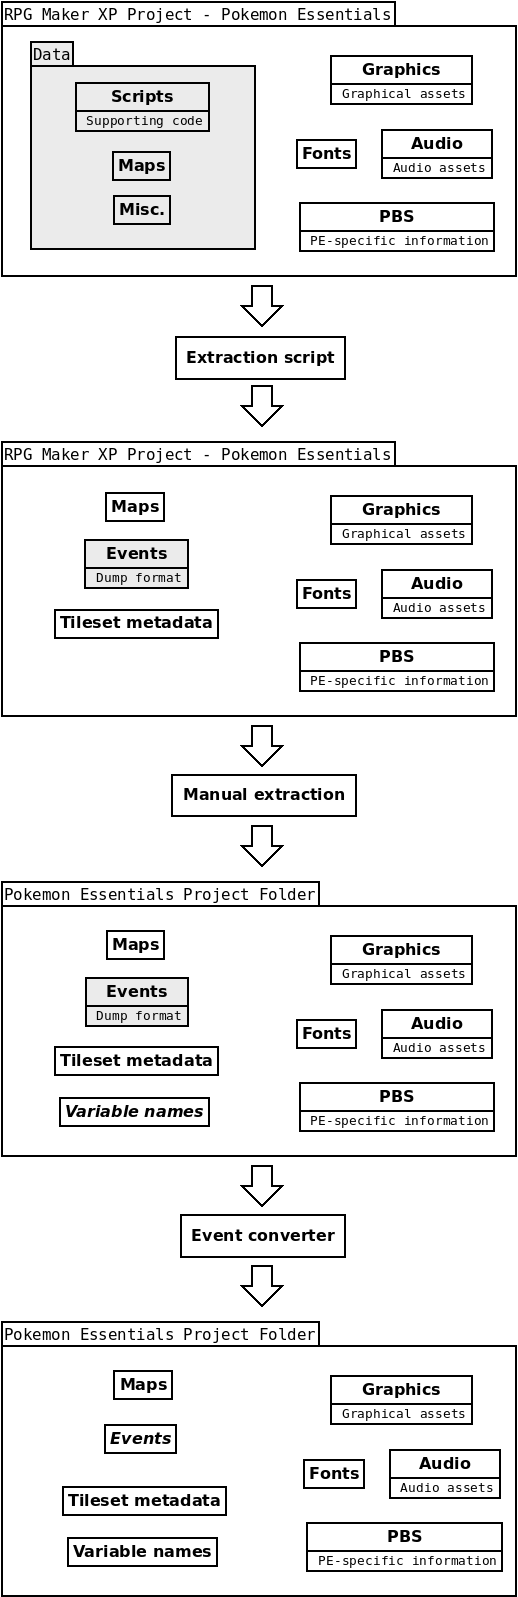
\includegraphics[width=1\linewidth]{Steps}
	\end{center}
\end{wrapfigure}


Pokemon Essentials, and other RPG Maker XP projects, have a clearly defined and standardized structure. Assets and data that make the content and logic of the game come in various formats, but for PoGER's purpose there is one important distinction :

\begin{itemize}
	\item Readily accessible data : Represented with white background, they exist in a standard format that can be interpreted/read without using RPG Maker XP.
	
	\item Obfuscated data : Represented with gray background, they are typically compiled and need the RPG Maker XP engine to interpret them.
\end{itemize}

PoGER's extraction effort aims to retrieve \textit{obfuscated data} and give it a standardized representation for use outside RPG Maker XP.

You can find detailed information about this process in \verb|Extraction.pdf|.

\vspace{2mm}
\textbf{Extraction script}

This script needs to be integrated to the game and executed. It does most of the heavy lifting, extracting \textbf{Maps}, \textbf{Events} (though only dumps them for further processing) and \textbf{Tileset metadata}.

\vspace{2mm}
\textbf{Manual extraction}

Unfortunately, no other way of retrieving the names associated with in-game variables and switches was found. They are needed because working with variable names is easier than with integer IDs.

\vspace{2mm}
\textbf{Event converter}

Events are surprisingly complex elements in RPG Maker XP, and the need for a new representation drove the development of an utility dedicated to that process.

Events are converted to a \textbf{domain-specific language} (documented in \verb|RMXP doc.png|) and packaged into individual files and easily editable.

\vspace{2mm}
\textbf{Final result}

At the end of the extraction process, all assets and data used by the game exist in a RMXP-independent form.

This means that it's now possible for a third-party interpreter to run the game just like it ran on RPG Maker XP's !


\newpage
\section{Implementations}

\subsection{RPG Maker XP extraction script}

This extracts data from compiled files in the \verb|Data| directory.

It can be found at \verb|RMXP_research/Extraction script/Extraction.rb|. Please read \verb|Extraction.pdf| for usage instructions.

In the same directory, you can find old versions of the same script and an attempt at a PBS-extraction script I wrote before realizing I was reinventing the wheel.

It was tested on both \textbf{Pokemon Essentials} and \textbf{Pokemon Uranium}.

\subsection{Event converter}

This converts events from their "JSON dump" representation to a human-readable format.

It can be found at \verb|RMXP_research/Event converter/Event_reader.py|.

Features :
\begin{itemize}
	\item Extracts events into individual files.
	\item Translates events to domain-specific language.
	\item Lists scripts called by events for ease of implementation.
\end{itemize}

Note : \verb|RGSS_Command_conversion.py| contains a translation function for every event command and {\ttfamily PE\_vari-
ables\_switches.py} contains dictionaries for variable/switch names.

\subsection{Map reader}

This reads an map from its own file and its tileset/autotiles assets files and reconstructs it.

It can be found at \verb|RMXP_research/Autotile research/LoadMap.py|. 

Features :
\begin{itemize}
	\item Can process multiple maps from a list.
	\item Implements a map reader class.
	\item Can decode both \textbf{Tilesets} and \textbf{Autotiles}.
	\item Has the ability to output \textbf{static} and \textbf{animated} maps.
	\item Useless beta feature : Reducing tilesets according to the specific needs of a particular map. 
\end{itemize}

\subsection{Interpreter}

This executes an event from its file.

It can be found at \verb|RMXP_research/Interpreter/eventReader.py|. 

Other files :
\begin{itemize}
	\item \verb|Interpreter| : Interprets events DSL
	\item \verb|pbInterpreter| : Interprets events script calls.
\end{itemize}

\subsection{PBS reader}

This loads data from PBS files and stores it for further use by game's logic.

It can be found at \verb|RMXP_research/PBSreader/|. 

\subsection{Demo}

TODO


\newpage
\section{Remarks}

\subsection{Contact}

Contact the author by email : \href{mailto:David.Rodriguez.1@etu.unige.ch}{David.Rodriguez.1@etu.unige.ch}



\end{document}